\documentclass[12pt]{article}
\usepackage{amsmath}
\usepackage{latexsym}
\usepackage{amsfonts}
\usepackage[normalem]{ulem}
\usepackage{soul}
\usepackage{array}
\usepackage{amssymb}
\usepackage{extarrows}
\usepackage{graphicx}
\usepackage[backend=biber,
style=numeric,
sorting=none,
isbn=false,
doi=false,
url=false,
]{biblatex}\addbibresource{bibliography.bib}

\usepackage{subfig}
\usepackage{wrapfig}
\usepackage{wasysym}
\usepackage{enumitem}
\usepackage{adjustbox}
\usepackage{ragged2e}
\usepackage[svgnames,table]{xcolor}
\usepackage{tikz}
\usepackage{longtable}
\usepackage{changepage}
\usepackage{setspace}
\usepackage{hhline}
\usepackage{multicol}
\usepackage{tabto}
\usepackage{float}
\usepackage{multirow}
\usepackage{makecell}
\usepackage{fancyhdr}
\usepackage[toc,page]{appendix}
\usepackage[hidelinks]{hyperref}
\usetikzlibrary{shapes.symbols,shapes.geometric,shadows,arrows.meta}
\tikzset{>={Latex[width=1.5mm,length=2mm]}}
\usepackage{flowchart}\usepackage[paperheight=11.69in,paperwidth=8.27in,left=1.0in,right=0.77in,top=1.0in,bottom=1.0in,headheight=1in]{geometry}
\usepackage[utf8]{inputenc}
\usepackage[T1]{fontenc}
\TabPositions{0.5in,1.0in,1.5in,2.0in,2.5in,3.0in,3.5in,4.0in,4.5in,5.0in,5.5in,6.0in,}

\urlstyle{same}

\renewcommand{\_}{\kern-1.5pt\textunderscore\kern-1.5pt}


\setcounter{tocdepth}{5}
\setcounter{secnumdepth}{5}


\setlistdepth{9}
\renewlist{enumerate}{enumerate}{9}
		\setlist[enumerate,1]{label=\arabic*)}
		\setlist[enumerate,2]{label=\alph*)}
		\setlist[enumerate,3]{label=(\roman*)}
		\setlist[enumerate,4]{label=(\arabic*)}
		\setlist[enumerate,5]{label=(\Alph*)}
		\setlist[enumerate,6]{label=(\Roman*)}
		\setlist[enumerate,7]{label=\arabic*}
		\setlist[enumerate,8]{label=\alph*}
		\setlist[enumerate,9]{label=\roman*}

\renewlist{itemize}{itemize}{9}
		\setlist[itemize]{label=$\cdot$}
		\setlist[itemize,1]{label=\textbullet}
		\setlist[itemize,2]{label=$\circ$}
		\setlist[itemize,3]{label=$\ast$}
		\setlist[itemize,4]{label=$\dagger$}
		\setlist[itemize,5]{label=$\triangleright$}
		\setlist[itemize,6]{label=$\bigstar$}
		\setlist[itemize,7]{label=$\blacklozenge$}
		\setlist[itemize,8]{label=$\prime$}


\pagestyle{fancy}
\fancyhf{}
\cfoot{ 
\vspace{\baselineskip}
}
\renewcommand{\headrulewidth}{0pt}
\setlength{\topsep}{0pt}\setlength{\parindent}{0pt}



\renewcommand{\arraystretch}{1.3}



\begin{document}

\vspace{\baselineskip}
\begin{Center}
{\fontsize{18pt}{21.6pt}\selectfont \textbf{\ \ \  Session Hijacking Attack On Whatsapp}\par}
\end{Center}\par

\begin{adjustwidth}{2.0in}{0.0in}
\begin{Center}
{\fontsize{18pt}{21.6pt}\selectfont \textbf{(Exploiting QR-Code Login)\tab \tab \tab \tab }\par}
\end{Center}\par

\end{adjustwidth}

\begin{FlushLeft}
{\fontsize{16pt}{19.2pt}\selectfont \textbf{ \tab \tab \tab \tab Himanshu Gwalani}\par}
\end{FlushLeft}\par

\begin{adjustwidth}{2.0in}{0.0in}
\begin{FlushLeft}
{\fontsize{16pt}{19.2pt}\selectfont \textbf{\ \  (2017UCP1356)}\par}
\end{FlushLeft}\par

\end{adjustwidth}


\vspace{\baselineskip}
\begin{adjustwidth}{1.0in}{0.0in}
\begin{FlushLeft}
{\fontsize{14pt}{16.8pt}\selectfont \textbf{\  CST 308 - Computer Network and Security}\par}
\end{FlushLeft}\par

\end{adjustwidth}

\begin{Center}
{\fontsize{14pt}{16.8pt}\selectfont \textbf{Malaviya National Institute of Technology, Jaipur}\par}
\end{Center}\par


\vspace{\baselineskip}

\vspace{\baselineskip}

\vspace{\baselineskip}

\vspace{\baselineskip}

\vspace{\baselineskip}

\vspace{\baselineskip}

\vspace{\baselineskip}

\vspace{\baselineskip}

\vspace{\baselineskip}

\vspace{\baselineskip}

\vspace{\baselineskip}

\vspace{\baselineskip}

\vspace{\baselineskip}

\vspace{\baselineskip}

\vspace{\baselineskip}

\vspace{\baselineskip}

\vspace{\baselineskip}

\vspace{\baselineskip}

\vspace{\baselineskip}

\vspace{\baselineskip}

\vspace{\baselineskip}

\vspace{\baselineskip}

\vspace{\baselineskip}

\vspace{\baselineskip}

\vspace{\baselineskip}

\vspace{\baselineskip}

\vspace{\baselineskip}

\vspace{\baselineskip}

\vspace{\baselineskip}

\vspace{\baselineskip}

\vspace{\baselineskip}

\vspace{\baselineskip}

\vspace{\baselineskip}

\vspace{\baselineskip}

\vspace{\baselineskip}
\begin{FlushLeft}
{\fontsize{18pt}{21.6pt}\selectfont \textbf{1\ \ \  Introduction }\par}
\end{FlushLeft}\par

\begin{FlushLeft}
This project consists of three modules :
\end{FlushLeft}\par

\begin{itemize}
	\item \textbf{Him’s Bot} :This tool is a social engineering attack vector which could be used for session hijacking over websites which implement \textbf{QR} code as \textbf{Login} functionality. It establishes a connection with web.whatsapp.com and synchronizes the QR code with that on the phishing page. As the victim scans the code, it saves the exchanged information between phone and website. This information includes a \textbf{secret key}, \textbf{webId}(of browser’s tab)\textbf{, version }of browser, \textbf{location}, \textbf{type of OS}, etc (in JSON), and it is used for login from the attacker's system but disguised as the victim.\par

	\item \textbf{Face Authentication} : The above bot is secured using face-lock mechanism, i.e. the bot will only execute when authenticated with my face.\par

	\item \textbf{Email Sender} : This is used to bait the user with a mail containing a link to the phishing page.
\end{itemize}\par

\begin{FlushLeft}
Web whatsapp exchanges information with the phone as a \textbf{client-server model}, where the \textbf{phone} acts as a \textbf{server} while the \textbf{website }acts\textbf{ }as a \textbf{client}. We bait the victim by sending a mail which includes a link to a phishing page containing QR code. This page is synchronized with web.whatsapp.com(using python scripts). Whatsapp reloads QR code every 15 seconds. The code is also reloaded on the phishing page. As the user scans it, the secret key (magic number) is captured by the \textbf{bot}, which is further used for login to \textbf{web.whatsapp.com} disguised as victim. 
\end{FlushLeft}\par

\begin{FlushLeft}
The major challenge is to synchronize the QR code (script on attacker’s side).
\end{FlushLeft}\par


\vspace{\baselineskip}
\begin{FlushLeft}
{\fontsize{18pt}{21.6pt}\selectfont \textbf{2}\ \ \  \textbf{Login with QR code}\par}
\end{FlushLeft}\par

\begin{FlushLeft}
Authentication over most of platform’s is dependent on traditional (id-password) based system. The credential system is dominating over others but with a few shortcomings like replay or phishing attack, password fatigue (remember password for multiple applications), etc. To eradicate those came SSO (single sign on) which is based on a single (id-password) pair for multiple services like google account. Then was introduced QR based login.
\end{FlushLeft}\par

\begin{FlushLeft}
\textcolor[HTML]{24292E}{In a QR-code-based login, a user may only need to scan a QR code generated by the service he’s trying to authenticate to, and then a client app on a trusted device such as a smartphone would scan and transmit the QR code to an identity provider in order to validate it and further authenticate the user to the destination service. }
\end{FlushLeft}\par

\begin{FlushLeft}
\textcolor[HTML]{24292E}{There could be several ways to authenticate using QR code :}
\end{FlushLeft}\par

\begin{enumerate}
	\item \textcolor[HTML]{24292E}{The QR code may contain the URL of the server website, and when phone scan the QR code, it will transmit the device id (may be phone number), etc information to the server. The server will be notified that the account credentials linked with the device need to be shared with the corresponding website.}\par

	\item \textcolor[HTML]{24292E}{The mobile device can also transfer stored credentials directly to website.}
\end{enumerate}\par

\begin{FlushLeft}
In this project I have exploited this login functionality over \textbf{whatsapp .}
\end{FlushLeft}\par


\vspace{\baselineskip}

\vspace{\baselineskip}
\begin{FlushLeft}
{\fontsize{18pt}{21.6pt}\selectfont \textbf{3\ \ \  Process Flow of Attack}\par}
\end{FlushLeft}\par

\begin{enumerate}
	\item \textbf{Face Authentication} : This is required to begin execution of him’s bot. This includes a python script for face detection and matching with existing information of my face stored as \textbf{flattened numpy array in text file}.\par

\begin{FlushLeft}
It\ uses  KNN ( K Nearest Neighbour ) algorithm for matching of the face.
\end{FlushLeft}\par

\begin{FlushLeft}
\textbf{KNN} : It is a supervised machine learning algorithm that can be used to solve both classification and regression problems.
\end{FlushLeft}\par

\begin{FlushLeft}
\textbf{Hyper-parameter} : k=5, distance formulae = ‘euclid’s distance’
\end{FlushLeft}\par

\begin{FlushLeft}
\textbf{$\#$  s is test data}
\end{FlushLeft}\par

\begin{FlushLeft}
\textbf{KNN(s):}
\end{FlushLeft}\par

\begin{FlushLeft}
\tab For each training data (tr):
\end{FlushLeft}\par

\begin{FlushLeft}
\ \ \ \ \ \ \ \ \ \  \tab -\  Calculate distance between s and tr.
\end{FlushLeft}\par

\begin{FlushLeft}
\tab \tab -\  Add this distance with label of s in ordered set
\end{FlushLeft}\par

\begin{FlushLeft}
\tab \tab -\  Sort the set in non-decreasing order
\end{FlushLeft}\par

\begin{FlushLeft}
\tab \tab -\  Get the labels of first ‘k’ entries
\end{FlushLeft}\par

\begin{FlushLeft}
-\  return \textbf{mode} of those k classes
\end{FlushLeft}\par

\begin{FlushLeft}
\textbf{end KNN}
\end{FlushLeft}\par

\begin{FlushLeft}
\textbf{Advantages:}
\end{FlushLeft}\par

\begin{enumerate}
	\item It is simple easy to implement.\par

	\item No assumptions, or training of model is required.\par

	\item The algorithm is versatile. It can be used for classification, regression and search.
\end{enumerate}\par

\begin{FlushLeft}
\textbf{Disadvantages}:
\end{FlushLeft}\par

\begin{enumerate}
	\item The algorithm gets significantly slower as the number of examples and/or predictors/independent variables increase.
\end{enumerate}\par

\begin{FlushLeft}
\textbf{In this module, no scientific python library was used. KNN algorithm was implemented using naive python.}
\end{FlushLeft}\par


\vspace{\baselineskip}

\vspace{\baselineskip}
	\item \textbf{Setting up attack environment} :\par

\begin{FlushLeft}
Post authentication, him’s bot will begin execution.
\end{FlushLeft}\par

\begin{itemize}
	\item The bot will initialize a client side QR session. This will setup a connection with web.whatsapp.com. The site will respond as a web-page containing QR code. Bot will extract the QR code and initialize an ONCHANGE Listener over it. This QR will be cloned to our phishing\_page.html. This will synchronize web.whatsapp’s QR with phishing\_page QR code. \par

	\item After this, the phishing website will be hosted on attacker’s (our) system on port specified by the command line.
\end{itemize}\par


\vspace{\baselineskip}
	\item \textbf{Initialize attack} :\par

After phishing website is hosted, an email is sent to the victim.The mail includes a link to the phishing page.As the victim clicks on it, he will be directed to the attacker’s(our) website. This will be having the QR code. Victim will scan the QR code. This is done using the \textbf{smtplib} library of python. Features : \textbf{smtp\_host} = ‘smtp.gmail.com’, \textbf{smtp\_port} = 587, \par

\textbf{victim’s email} : input\par


\vspace{\baselineskip}
	\item \textbf{Capture session information} : After victim scans the code, the phone will transmit data (magic number, location, etc.) to the server, and further the server will send the authentication credentials to our website. This information will be saved to our system in \textbf{JSON} format at /session/id.\par


\vspace{\baselineskip}



\begin{figure}[H]
	\begin{FlushLeft}		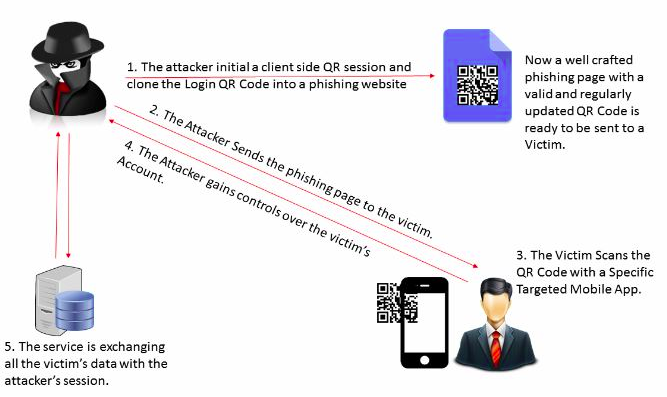
\includegraphics[width=6.88in,height=3.2in]{./media/image1.png}
	\end{FlushLeft}\end{figure}



\par


\vspace{\baselineskip}
	\item \textbf{Starting victim’s session}:
\end{enumerate}\par

\begin{adjustwidth}{0.5in}{0.0in}
\begin{FlushLeft}
\textbf{Command} : sessions -i ‘s\_id’
\end{FlushLeft}\par

\end{adjustwidth}

\begin{adjustwidth}{0.5in}{0.0in}
\begin{FlushLeft}
This will initiate the session with id = ‘s\_id’. This will be done by him’s bot. It will open firefox with url as web.whatsapp.com. As the page appears, it will provide stored credentials for the corresponding victim. Since whatsapp uses same (magic number) until it’s session is ended manually from phone or desktop we will be able to access the victim's account even after restarting the browser. The only requirement is to keep the victim’s phone connected to the internet, since it is specified by whatsapp.
\end{FlushLeft}\par

\end{adjustwidth}

\begin{adjustwidth}{0.0in}{-0.19in}
And now, the victim’s account is hijacked.\par

\end{adjustwidth}


\vspace{\baselineskip}
\begin{FlushLeft}
{\fontsize{18pt}{21.6pt}\selectfont \textbf{4\ \ \  ClickJacking vs QR code Hijacking}\par}
\end{FlushLeft}\par

\begin{FlushLeft}
Clickjacking, also known as a $``$\textbf{UI redress attack}$"$ , is when an attacker uses multiple transparent or opaque layers to trick a user into clicking on a button or link on another page, when the user wants to click on the top level page.
\end{FlushLeft}\par

\begin{FlushLeft}
However, clickjacking will \textbf{not} be able to surpass \textbf{2-step verification}.
\end{FlushLeft}\par

\begin{FlushLeft}
For example: If an attacker tries to somehow convince the victim to change email and password as per attacker, but if the authentication involves 2-step verification, the attacker would still won’t be able to hijack.
\end{FlushLeft}\par

\begin{FlushLeft}
On contrary, QR code login involves:
\end{FlushLeft}\par

\begin{itemize}
	\item SSO (Single Sign On) : use of the same credentials for multiple systems.\par

	\item 2-step verification
\end{itemize}\par

\begin{FlushLeft}
So QR code can be considered as the final defence line which provides usability and security. So QR code exploitation is more severe than normal clickjacking attacks.
\end{FlushLeft}\par


\vspace{\baselineskip}
\begin{FlushLeft}
{\fontsize{18pt}{21.6pt}\selectfont \textbf{5\ \ \  Defences}\par}
\end{FlushLeft}\par

\begin{FlushLeft}
Here are a few proposed defenses for QR based session hijacking attack:
\end{FlushLeft}\par

\begin{itemize}
	\item \textbf{Use of OTP (one time password)} : This would be best to implement instead of QR based Login. Since the requirement in both cases is a device (phone) which the user can trust. So it is an efficient and much secure authentication mechanism.\par

	\item \textbf{Session Confirmation} : Implementation of a confirmation notification displaying characteristic information about the session made by the client/server.\par

	\item Not allow authentication for different networks (WAN’s).\par

	\item \textbf{Audio based authentication}: After the user scans QR code, the device (phone) generates an audio which includes a message signed with the \textbf{private key} of the user. The website extracts the message using the \textbf{public key} of the user. If both messages are the same , authentication is successful. Using this, the attacker will not be able to extract the message and attack is unsuccessful.
\end{itemize}\par

\begin{FlushLeft}
{\fontsize{18pt}{21.6pt}\selectfont \textbf{6\ \ \  Conclusion}\par}
\end{FlushLeft}\par

\begin{FlushLeft}
In this project, I have successfully demonstrated QR based session hijacking over whatsapp. The vulnerability of QR based login mechanism is exploited by capturing the magic number (secret key) and other necessary information for session establishment. This also includes demonstration of face unlock using KNN algorithm. The technology stack mainly includes \textbf{python3}, \textbf{smtplib}, \textbf{JSON}.
\end{FlushLeft}\par

\begin{FlushLeft}
\textbf{Main learnings} of this project were implementation of KNN, extraction of session information using python scripts, synchronize web pages using threads, and communication between two applications (browser and him’s bot) using \textbf{geckodriver}.
\end{FlushLeft}\par

\begin{FlushLeft}
The current module of Him’s bot\textbf{ }only targets whatsapp, however it could be further extended to applications which use QR based login mechanisms like weChat, Yandex, etc.
\end{FlushLeft}\par


\vspace{\baselineskip}

\vspace{\baselineskip}
\begin{FlushLeft}
{\fontsize{18pt}{21.6pt}\selectfont \textbf{7\ \ \  References}\par}
\end{FlushLeft}\par

\begin{itemize}
	\item Mozilla developer resource on Content-Security-Policy frame-ancestors response header.\par

	\item \href{https://owasp.org/www-community/attacks/Clickjacking}{\textcolor[HTML]{1155CC}{\ul{https://owasp.org/www-community/attacks/Clickjacking}}}\par

	\item \href{https://brownglock.com/library/2016/08/02/qrljacking-attack-can-bypass-any-qr-login-system/}{\textcolor[HTML]{1155CC}{\ul{https://brownglock.com/library/2016/08/02/qrljacking-attack-can-bypass-any-qr-login-system/}}}\par

	\item \href{https://towardsdatascience.com/machine-learning-basics-with-the-k-nearest-neighbors-algorithm-6a6e71d01761}{\textcolor[HTML]{1155CC}{\ul{https://towardsdatascience.com/machine-learning-basics-with-the-k-nearest-neighbors-algorithm-6a6e71d01761}}}\par

	\item \href{https://stackoverflow.com/questions/8055132/python-sending-email-too-slow}{\textcolor[HTML]{1155CC}{\ul{https://stackoverflow.com/questions/8055132/python-sending-email-too-slow}}}
\end{itemize}\par


\printbibliography
\end{document}